\documentclass{beamer}
\usepackage[utf8]{inputenc}

\usetheme{Madrid}
\usecolortheme{default}
\usepackage{txfonts}
\usepackage{listings}
\usepackage{adjustbox}
\usepackage{tabularx}
\usepackage{lmodern}
\usepackage{circuitikz}
\usepackage{tikz}

\usepackage{gvv}
\usepackage{cite}
\usepackage{amsmath,amssymb,amsfonts,amsthm}
\usepackage{algorithmic}
\usepackage{graphicx}
\usepackage{textcomp}
\usepackage{xcolor}
\usepackage{txfonts}
\usepackage{listings}
\usepackage{enumitem}
\usepackage{mathtools}
\usepackage{gensymb}
\usepackage{comment}
\usepackage{tkz-euclide} 
\usepackage{listings}                                      
\def\inputGnumericTable{}                                
\usepackage{color}                                            
\usepackage{array}                                            
\usepackage{longtable}
\usepackage{multicol}
\usepackage{calc}                                             
\usepackage{multirow}                                         
\usepackage{hhline}                                           
\usepackage{ifthen}

\setbeamertemplate{page number in head/foot}[totalframenumber]

\usepackage{tcolorbox}
\tcbuselibrary{minted,breakable,xparse,skins}



\definecolor{bg}{gray}{0.95}
\DeclareTCBListing{mintedbox}{O{}m!O{}}{%
  breakable=true,
  listing engine=minted,
  listing only,
  minted language=#2,
  minted style=default,
  minted options={%
    linenos,
    gobble=0,
    breaklines=true,
    breakafter=,,
    fontsize=\small,
    numbersep=8pt,
    #1},
  boxsep=0pt,
  left skip=0pt,
  right skip=0pt,
  left=25pt,
  right=0pt,
  top=3pt,
  bottom=3pt,
  arc=5pt,
  leftrule=0pt,
  rightrule=0pt,
  bottomrule=2pt,
  toprule=2pt,
  colback=bg,
  colframe=orange!70,
  enhanced,
  overlay={
    \begin{tcbclipinterior}
    \fill[orange!20!white] (frame.south west) rectangle ([xshift=20pt]frame.north west);
    \end{tcbclipinterior}},
  #3,
}
\lstset{
    language=C,
    basicstyle=\ttfamily\small,
    keywordstyle=\color{blue},
    stringstyle=\color{orange},
    commentstyle=\color{green!60!black},
    numbers=left,
    numberstyle=\tiny\color{gray},
    breaklines=true,
    showstringspaces=false,
}

\title 
{4.11.9}
\date{October 1, 2025}


\author 
{Sai Sreevallabh - EE25BTECH11031}



\begin{document}


\frame{\titlepage}
\begin{frame}{Question}
Find the area of the triangle $\triangle ABC$ bounded by the lines $4x-y+5 = 0$, $x+y-5 = 0$ and $x-4y+5 = 0$. \\
\end{frame}



\begin{frame}{Theoretical Solution}

Given lines can be written as: 

\begin{align}
    \myvec{4&-1}\myvec{x\\y} = -5 \label{eq:1}
\end{align}

\begin{align}
    \myvec{1&1}\myvec{x\\y} = 5 \label{eq:2}
\end{align}

\begin{align}
    \myvec{1&-4}\myvec{x\\y} = -5 \label{eq:3}
\end{align}

\end{frame}

\begin{frame}{Theoretical Solution}

Solving equations \eqref{eq:1} and \eqref{eq:2} to get the point of intersection $\vec{A}$:

\begin{align}
    \myvec{1&1\\4&-1}\myvec{x\\y} =& \myvec{5\\-5}
\end{align}

Making the Augmented Matrix and converting to echelon form

\begin{align}
    \augvec{2}{1}{1&1&5\\4&-1&-5} \xleftrightarrow[]{R_2 \xrightarrow{} R_2-4R_1} \augvec{2}{1}{1&1&5\\0&-5&-25}
\end{align}

We get
\begin{align}
    \vec{A}=\myvec{0\\5}
\end{align}
\end{frame}

\begin{frame}{Theoretical Solution}
Solving equations \eqref{eq:2} and \eqref{eq:3} to get the point of intersection $\vec{B}$

\begin{align}
    \augvec{2}{1}{1&1&5\\1&-4&-5} \xleftrightarrow[]{R_2 \xrightarrow{} R_2-R_1} \augvec{2}{1}{1&1&5\\0&-5&-10}
\end{align}

We get
\begin{align}
    \vec{B}= \myvec{3\\2}
\end{align}

\end{frame}

\begin{frame}{Theoretical Solution}
Solving equations \eqref{eq:1} and \eqref{eq:3} to get the point of intersection $\vec{C}$

\begin{align}
    \augvec{2}{1}{1&-4&-5\\4&-1&5} \xleftrightarrow[]{R_2 \xrightarrow{} R_2-4R_1} \augvec{2}{1}{1&-4&-5\\0&15&15}
\end{align}

We get
\begin{align}
    \vec{C}= \myvec{-1\\1}
\end{align}
\end{frame}

\begin{frame}{Theoretical Solution}
   The vertices of the triangle are

\begin{align}
    \vec{A}=\myvec{0\\5} \ ,\ \vec{B}= \myvec{3\\2} \ , \ \vec{C}= \myvec{-1\\1}
\end{align}

Now

\begin{align}
    \vec{B-A} = \myvec{3\\-3} \ \text{and} \ \vec{C-A} = \myvec{-1\\-4}
\end{align}\\

% Area of the triangle $\triangle ABC$ is given by
% \begin{align}
%     \frac{1}{2}\norm{\brak{\vec{B-A}}\times\brak{\vec{C-A}}}
% \end{align}
\end{frame}

\begin{frame}{Theoretical Solution}
    Area of the triangle $\triangle ABC$ is given by
\begin{align}
    \frac{1}{2}\norm{\brak{\vec{B-A}}\times\brak{\vec{C-A}}}
\end{align}

\begin{align}
    =&\ \ \frac{1}{2}\norm{\myvec{3\\-3}\times\myvec{-1\\-4}}\\
    =&\ \ \frac{15}{2}
\end{align}

Hence,
\begin{align}
    ar\brak{\triangle ABC} = \frac{15}{2}
\end{align}\\

% $\therefore$ The area of the triangle formed by the given three lines is $\frac{15}{2}$ units. 
\end{frame}


\begin{frame}[fragile]
    \frametitle{C Code - Finding x-coordinate of Point of Intersection}

    \begin{lstlisting}

#include <stdio.h>
#include <math.h>

double POI_x(double a1, double b1, double c1, double a2, double b2, double c2){
   
    double x = (b1*c2-b2*c1)/(a1*b2-a2*b1);
   
    return x;
}

    \end{lstlisting}

\end{frame}

\begin{frame}[fragile]
    \frametitle{C Code - Finding y-coordinate of Point of Intersection}

    \begin{lstlisting}

double POI_y(double a1, double b1, double c1, double a2, double b2, double c2){
   
    double y = (a2*c1-a1*c2)/(a1*b2-a2*b1);
   
    return y;
}

    \end{lstlisting}

\end{frame}


\begin{frame}[fragile]
    \frametitle{Python Code - Using Shared Object}
    \begin{lstlisting}
import numpy as np
import numpy.linalg as LA
import matplotlib.pyplot as plt
import ctypes

c_lib=ctypes.CDLL('./code.so')

c_lib.POI_x.argtypes = [ctypes.c_double, ctypes.c_double, ctypes.c_double, ctypes.c_double, ctypes.c_double,ctypes.c_double]

c_lib.POI_y.argtypes = [ctypes.c_double, ctypes.c_double, ctypes.c_double, ctypes.c_double, ctypes.c_double,ctypes.c_double]

c_lib.POI_x.restype = ctypes.c_double
c_lib.POI_y.restype = ctypes.c_double

\end{lstlisting}
\end{frame}

\begin{frame}[fragile]
    \frametitle{Python Code - Using Shared Object}
    \begin{lstlisting}


a1, b1, c1 = 4.0, -1.0, 5.0
a2, b2, c2 = 1.0, 1.0, -5.0
a3, b3, c3 = 1.0, -4.0, 5.0

x1 = c_lib.POI_x(a1, b1, c1, a2, b2, c2)
y1 = c_lib.POI_y(a1, b1, c1, a2, b2, c2)

x2 = c_lib.POI_x(a2, b2, c2, a3, b3, c3)
y2 = c_lib.POI_y(a2, b2, c2, a3, b3, c3)

x3 = c_lib.POI_x(a3, b3, c3, a1, b1, c1)
y3 = c_lib.POI_y(a3, b3, c3, a1, b1, c1)

\end{lstlisting}
\end{frame}

\begin{frame}[fragile]
    \frametitle{Python Code - Using Shared Object}
    \begin{lstlisting}
    
A = np.array([x1, y1])
B = np.array([x2, y2])
C = np.array([x3, y3])

plt.plot([A[0],B[0]],[A[1],B[1]], label = "$4x-y+5=0$")
plt.plot([C[0],B[0]],[C[1],B[1]], label = "$x+y-5=0$")
plt.plot([A[0],C[0]],[A[1],C[1]], label = "$x-4y+5=0$")

A = A.reshape(-1,1)
B = B.reshape(-1,1)
C = C.reshape(-1,1)


\end{lstlisting}
\end{frame}

\begin{frame}[fragile]
    \frametitle{Python Code - Using Shared Object}
    \begin{lstlisting}
tri_coords = np.block([[A,B,C]])
plt.scatter(tri_coords[0,:], tri_coords[1,:])
vert_labels = ['A','B','C']

for i, txt in enumerate(vert_labels):
    plt.annotate(f'{txt}\n({tri_coords[0,i]:.0f}, {tri_coords[1,i]:.0f})',
                 (tri_coords[0,i], tri_coords[1,i]), 
                 textcoords="offset points", 
                 xytext=(20,5), 
                 ha='center') 

    \end{lstlisting}
    
\end{frame}

\begin{frame}[fragile]
    \frametitle{Python Code - Using Shared Object}
    \begin{lstlisting}
    
ax = plt.gca()
ax.spines['top'].set_color('none')
ax.spines['left'].set_position('zero')
ax.spines['right'].set_color('none')
ax.spines['bottom'].set_position('zero')
plt.xlabel('$x$')
plt.ylabel('$y$')
plt.legend(loc='best')
plt.grid() 
plt.axis('equal')

plt.savefig("../Figs/plot(py+C).png")

plt.show()

\end{lstlisting}
\end{frame}

\begin{frame}{Plot-Using Both C and Python}
    \centering
    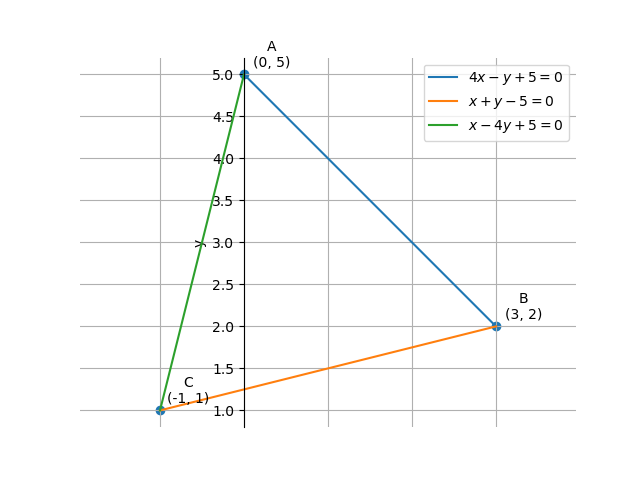
\includegraphics[width=\columnwidth, height=0.8\textheight, keepaspectratio]{Figs/plot(py+C).png}     
\end{frame}

%-------End of Python+C-------------


\begin{frame}[fragile]
    \frametitle{Python Code}
    \begin{lstlisting}
import math
import numpy as np
import matplotlib.pyplot as plt
import numpy.linalg as LA

a1, b1, c1 = 4.0, -1.0, 5.0
a2, b2, c2 = 1.0, 1.0, -5.0
a3, b3, c3 = 1.0, -4.0, 5.0

x1 = (b1*c2-b2*c1)/(a1*b2-a2*b1)
y1 = (a2*c1-a1*c2)/(a1*b2-a2*b1)

x2 = (b2*c3-b3*c2)/(a2*b3-a3*b2) 
y2 = (a3*c2-a2*c3)/(a2*b3-a3*b2)

x3 = (b1*c3-b3*c1)/(a1*b3-a3*b1)
y3 = (a3*c1-a1*c3)/(a1*b3-a3*b1)

\end{lstlisting}
\end{frame}

\begin{frame}[fragile]
    \frametitle{Python Code}
    \begin{lstlisting}

A = np.array([x1, y1])
B = np.array([x2, y2])
C = np.array([x3, y3])

plt.plot([A[0],B[0]],[A[1],B[1]], 'r', label = "$4x-y+5=0$")
plt.plot([C[0],B[0]],[C[1],B[1]], 'g', label = "$x+y-5=0$")
plt.plot([A[0],C[0]],[A[1],C[1]], 'b', label = "$x-4y+5=0$")

A = A.reshape(-1,1)
B = B.reshape(-1,1)
C = C.reshape(-1,1)

\end{lstlisting}
\end{frame}

\begin{frame}[fragile]
    \frametitle{Python Code}
    \begin{lstlisting}

tri_coords = np.block([[A,B,C]])
plt.scatter(tri_coords[0,:], tri_coords[1,:])
vert_labels = ['A','B','C']
for i, txt in enumerate(vert_labels):
    plt.annotate(f'{txt}\n({tri_coords[0,i]:.0f}, {tri_coords[1,i]:.0f})',
                 (tri_coords[0,i], tri_coords[1,i]), 
                 textcoords="offset points", 
                 xytext=(20,5), 
                 ha='center') 

\end{lstlisting}
\end{frame}

\begin{frame}[fragile]
    \frametitle{Python Code}
    \begin{lstlisting}
ax = plt.gca()
ax.spines['top'].set_color('none')
ax.spines['bottom'].set_position('zero')
ax.spines['right'].set_color('none')
ax.spines['left'].set_position('zero')
plt.xlabel('x')
plt.ylabel('y')
plt.legend(loc='best')
plt.grid()
plt.axis('equal')

plt.savefig("../Figs/plot(py).png")
plt.show()



    \end{lstlisting}
\end{frame}


\begin{frame}{Plot-Using Python only}
    \centering
    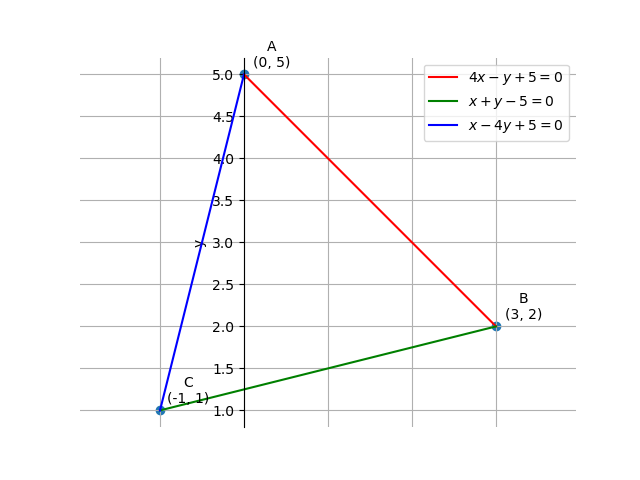
\includegraphics[width=\columnwidth, height=0.8\textheight, keepaspectratio]{Figs/plot(py).png}     
\end{frame}


\end{document}
